\chapter{Detalles de Implementación}\label{cap4}

La parte esencial de este trabajo esta dado por llevar a cabo una 
implementación que refleje el diseño propuesto en el capitulo anterior, 
brindando así una herramienta real a la comunidad que permita la comunicación 
anónima entre distintas partes interesadas.

Como fue explicado anteriormente, no existen muchas implementaciones de 
protocolos basados en DC-Net, por lo que llevar a cabo este trabajo conllevó 
soslayar muchos obstáculos que se detallan a continuación.

\section{Tecnologías Involucradas}

\begin{enumerate}
    \item \underline{Lenguaje de Programación:} para llevar a cabo este 
    proyecto se escogió realizarlo en \emph{Java}, debido principalmente a que 
    un objetivo era poder realizar una aplicación móvil como prueba de 
    concepto de lo implementado, y el sistema operativo móvil más común hoy en 
    día es \emph{Android}\footnote{\url{http://www.idc.com/promo/smartphone-market-share/os}}, el 
    cual está basado en \emph{Java}. No existe una razón de fondo (mayor \emph{
    performance} o expresividad del lenguaje), por el que se escogió \emph{Java
    }, por lo que los mismos resultados se pueden lograr si se utiliza otro 
    lenguaje más común en otras implementaciones de DC-Net, como sería \emph{
    C++}.

    \item \underline{Capa de comunicación:} para la conexión entre las 
    distintas partes se utilizó \emph{ZeroMQ}, el cual es un \emph{framework} 
    de concurrencia, que permite desligarse de lidiar con problemas típicos de 
    mensajería distribuida (desconexiones, pérdida de datos, etc.) y 
    concentrarse únicamente en la lógica de la aplicación. En palabras de sus 
    autores, ``\emph{ZeroMQ} son sockets con esteroides''. Con \emph{ZeroMQ} 
    se simplifica la implementación de \emph{broadcasting} o conexiones punto 
    a punto entre los distintos participantes (ambos tipos de conexiones 
    necesarias para el protocolo).
\end{enumerate}

\section{Arquitectura del Sistema: Nodos Directorio y Participantes}

Un desafío importante a considerar en la implementación (y que el diseño del 
protocolo no se preocupa) es como cada participante descubre la locación del resto de los 
participantes que formarán parte del \emph{anonymity-set}. Para ello se tomó 
la decisión de contar, además de los nodos participantes, con un nodo 
Directorio. Este nodo funcionará como punto de entrada al \emph{anonymity-set} 
y será el responsable de informar la dirección IP de cada uno de los nodos 
participantes presentes en la sala. Además de esto, el nodo Directorio tiene 
como responsabilidad establecer los parámetros necesarios para correr el protocolo (número de 
participantes que admitirá la sala, valores públicos para realizar los \emph{commitments}, 
largo máximo de los mensajes a enviar, entre otros), por lo que también se vuelve 
un punto de control dentro del protocolo. Un aspecto importante es que todo lo que 
relaciona el protocolo con mantener anonimato (envío y verificaciones de 
demostraciones de seguridad) no pasa por el nodo Directorio, por lo que su 
incorporación no altera en nada la seguridad y privacidad del sistema.

\begin{figure}[H]
  \centering
    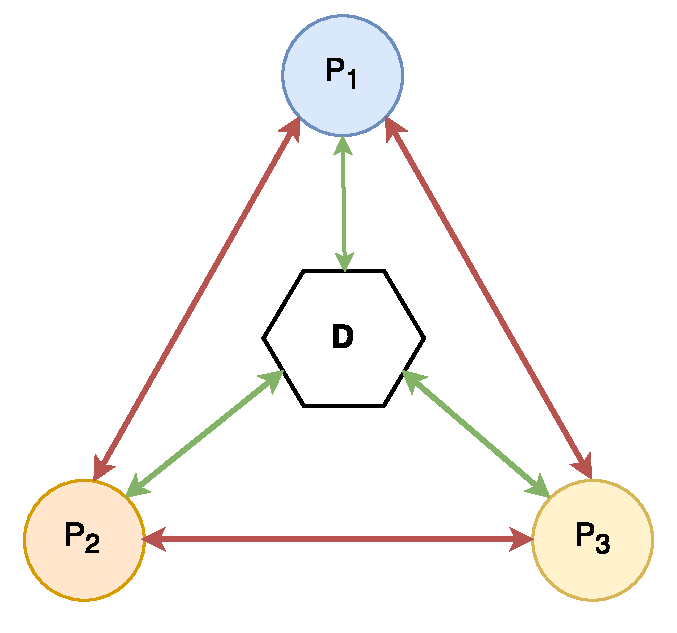
\includegraphics[width=0.5\textwidth]{imagenes/architecture.pdf}
  \caption{Conexión entre nodos Directorio y Participantes}
  \label{fig:connections-directory-participants}
\end{figure}

Esta tarea (punto de entrada a la sala) también se podría realizar entre los propios nodos participantes, 
sin la necesidad de incorporar un nodo Directorio. Si bien en esta 
investigación se priorizó la facilidad de implementar la variante utilizando 
el nodo adicional, se podría ejecutar alguna variante de \emph{gossip protocol} 
\cite{Demers:1987:EAR:41840.41841} 
para informar la identidad de participantes nuevos que vayan entrando a la sala, lo 
cual podría solucionar el problema. Esta segunda variante además tiene la ventaja 
de no poseer un punto vulnerable (que sería el nodo Directorio), evitando 
ataques directos al nodo Directorio, retrasando (o incluso imposibilitando) la 
creación del \emph{anonimity-set}. Reiterar que se implementó el nodo 
Directorio por simplicidad, pero se tienen en cuenta los posibles ataques que 
puede recibir el sistema, que no tienen incidencia en romper el anonimato que 
brinda el protocolo.

Actualmente el nodo Directorio inicializa estableciendo los parámetros 
públicos del protocolo y publica su dirección IP. Luego, cada nodo 
Participante que se quiera unir se conecta a la dirección pública del 
Directorio y espera que se complete la cuota de participantes establecida en 
un comienzo. Cuando se conectan los $n$ participantes necesarios al Directorio, éste informa 
la dirección IP de cada uno de los participantes a todo el resto, para que 
posteriormente inicien el protocolo solo enviándose mensajes entre ellos, 
finalizando así la labor del nodo Directorio. En la Figura \ref{fig:connections-directory-participants} 
se observa las conexiones que se realizan durante el desarrollo del protocolo, 
primero conectando cada participante que viene entrando a la sala al nodo 
Directorio (representado por las conexiones verdes), y luego que todos los 
participantes se hayan conectado al nodo Directorio, éste le comunica a toda 
la sala las direcciones de los nodos participantes presentes, terminando su labor, 
desconectándose de los nodos Participantes, y estos finalmente se conectan mediante 
los enlaces rojos entre cada uno de ellos. En la Figura \ref{fig:connections-participants} 
se observa en mayor detalle la conexión entre cada par de participantes, la 
cual se realiza a través de \emph{sockets} tipo \emph{requestor-replier}, formando 
así el \emph{anonimity-set} deseado, y continuando con el normal desarrollo 
del protocolo anteriormente descrito.

\begin{figure}[H]
  \centering
    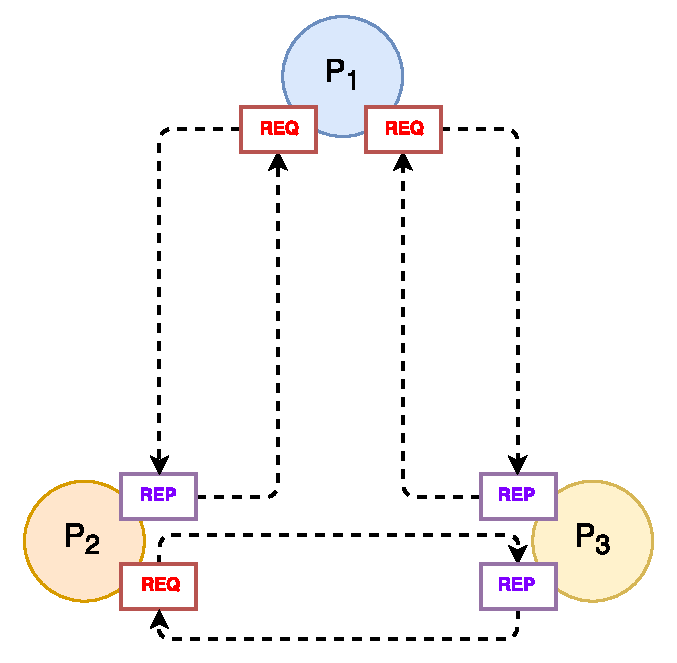
\includegraphics[width=0.5\textwidth]{imagenes/participants_connection.pdf}
  \caption{Conexión entre nodos participantes}
  \label{fig:connections-participants}
\end{figure}

\section{Primitivas Criptográficas}

En la implementación actual, la gran mayoría de las primitivas criptográficas 
han sido implementadas desde cero, valiéndose principalmente de la biblioteca 
para manejar números grandes de \emph{Java}, \emph{BigInteger}\footnote{\url{
https://docs.oracle.com/javase/7/docs/api/java/math/BigInteger.html}}. Si bien 
esto no es una práctica recomendada (lo ideal es utilizar bibliotecas 
criptográficas ya probadas por la comunidad), no se ha descubierto ninguna que 
se adecúe a las necesidades requeridas por el protocolo (\emph{Pedersen 
Commitments} y \emph{ZKP} asociadas). Este punto es algo importante a resolver 
ya que, como fue dicho, la implementación de primitivas criptográficas no es 
recomendado y es imperante utilizar implementaciones ya probadas y verificadas 
por la comunidad, como lo podría ser Charm-Crypto\footnote{\url{http://charm-
crypto.com/index.html}} o Scapi\footnote{\url{https://scapi.readthedocs.
io/en/latest/}}. De todas maneras, la criptografía implementada se desarrolló 
utilizando interfaces, por lo que cuando se descubra una librería que cumpla 
los requerimientos criptográficos que se buscan, su implantación sea realizada 
de manera expedita y transparente al resto de la implementación.

\section{\emph{API} implementada}

Como fue dicho anteriormente, una contribución importante de este trabajo 
sería el hecho de estar apuntado a implementar una \emph{API} disponible para 
toda la comunidad que quiera desarrollar una aplicación que esté basada en el 
protocolo anteriormente descrito. 

La implementación anterior fue empaquetada como librería \emph{Java}, 
utilizable por otras aplicaciones al importar el archivo \emph{.jar} generado. 
Esta librería quedó con los siguientes métodos de manera pública, formando así 
la \emph{API} disponible:

\begin{itemize}
    \item \texttt{DCNETProtocol class:} clase base que entrega la \emph{API} 
    que es necesario instanciar para utilizar los métodos descritos a 
    continuación. 
    \item \texttt{boolean connectToDirectory():} luego de setear la dirección 
    IP del nodo directorio, este método realiza la conexión desde el nodo partcipante
    hacia el directorio, utilizando las funciones provistas por la librería 
    \emph{ZeroMQ}.
    \item \texttt{void setMessageToSend(String s, boolean b):} este método tiene 
    como finalidad permitir al nodo participante establecer el mensaje que desea 
    comunicar al resto de la sala utilizando el protocolo. 
    \item \texttt{void runProtocol(PrintStream p):} corre el protocolo anteriormente 
    descrito de manera automática, calculando los diferentes \emph{commitments} y 
    \emph{zero-knowledge proofs} necesarios, repitiendo las rondas necesarios 
    y finalizando cuando todos los mensajes han sido recibidos por la totalidad 
    de los participantes en cuestión.
    \item \texttt{ObservableParticipantsLeft:} objeto que emplea el patrón de diseño 
    \emph{Observer} para ir informando cuáles participantes se van conectando a la sala 
    a medida que va ocurriendo, y así tener una noción de cuantos participantes faltan 
    para completar la cuota puesta en un principio por el nodo directorio.
    \item \texttt{ObservableMessagesArrived:} también emplea el patrón de diseño 
    \emph{Observer} para informar al participante de los mensajes que van resultando 
    de correr el protocolo, a medida que éste avanza. Despliega los mensajes en tiempo 
    real.
\end{itemize}

\section{Aplicación Móvil}

Para poder probar el uso de la \emph{API} implementada, se desarrolló una 
aplicación móvil prototipo, que tiene como objetivo permitir un uso simplificado 
del protocolo implementado, que permita a los usuarios montar una conversación 
que asegure el anonimato de sus participantes.

La aplicación está compuesta de 3 módulos: (1) conexión al nodo directorio, (2) envío 
del mensaje por parte del participante, y (3) recepción de los mensajes 
del resto de los participantes de la sala.

\begin{figure}[H]
    \centering
    \begin{subfigure}[b]{0.4\textwidth}
        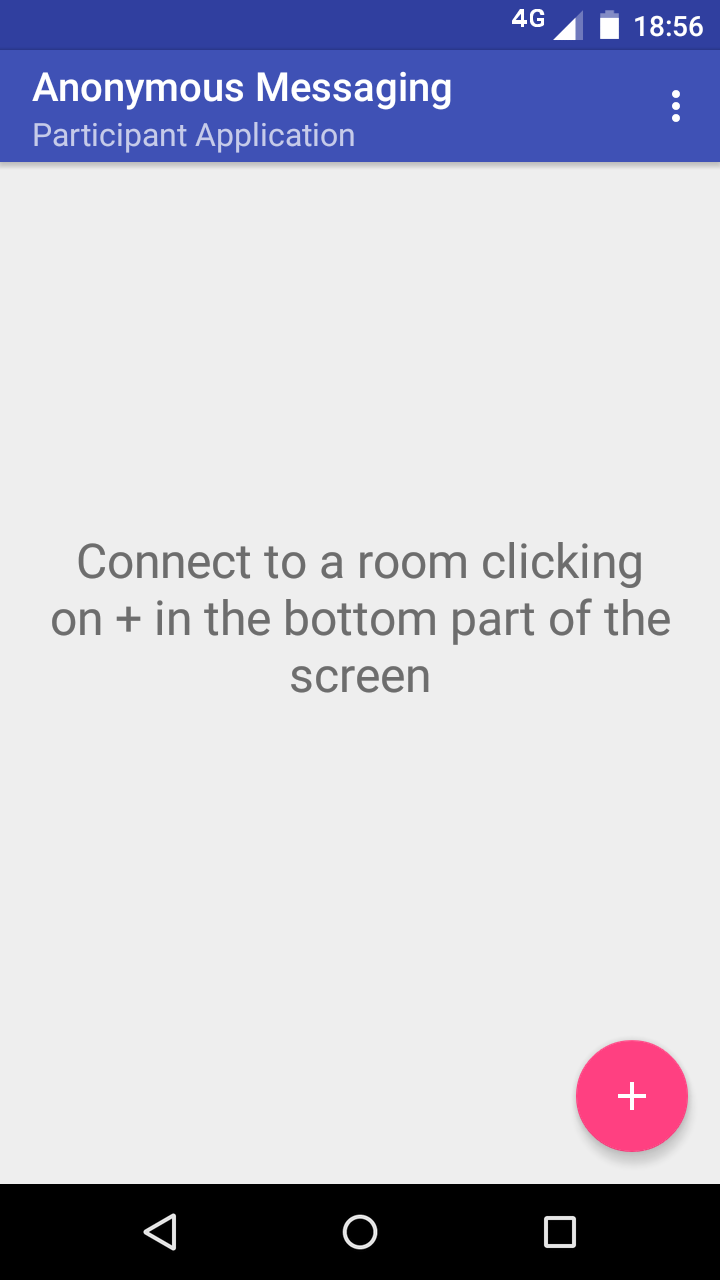
\includegraphics[width=\textwidth]{imagenes/mobile_first.png}
        \caption{Conexión al Nodo Directorio}
        \label{fig:mobile_connect}
    \end{subfigure}
    ~
    \begin{subfigure}[b]{0.4\textwidth}
        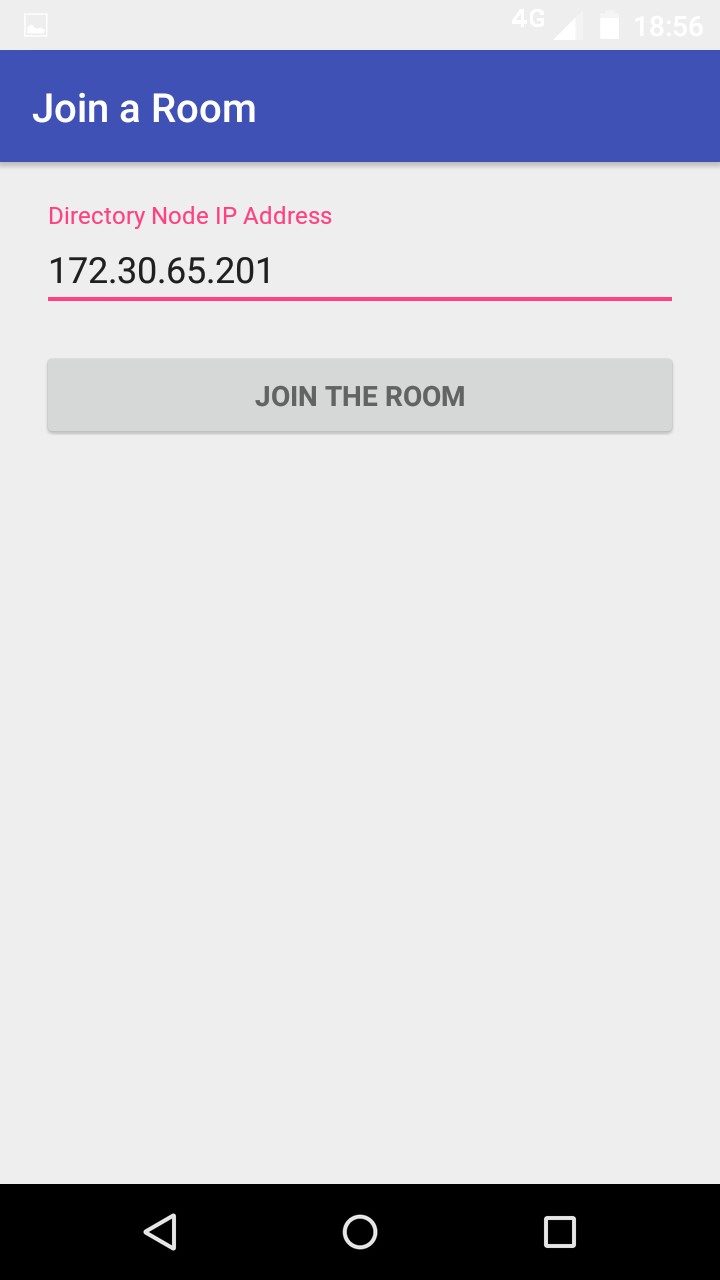
\includegraphics[width=\textwidth]{imagenes/mobile_connect.png}
        \caption{Establecer dirección del Directorio}
        \label{fig:mobile_set_ip}
    \end{subfigure}
    \caption{Screenshots de Aplicación Móvil (parte 1)}\label{fig:mobile_screenshots_1}
\end{figure}

\begin{figure}[H]
    \centering
    \begin{subfigure}[b]{0.4\textwidth}
        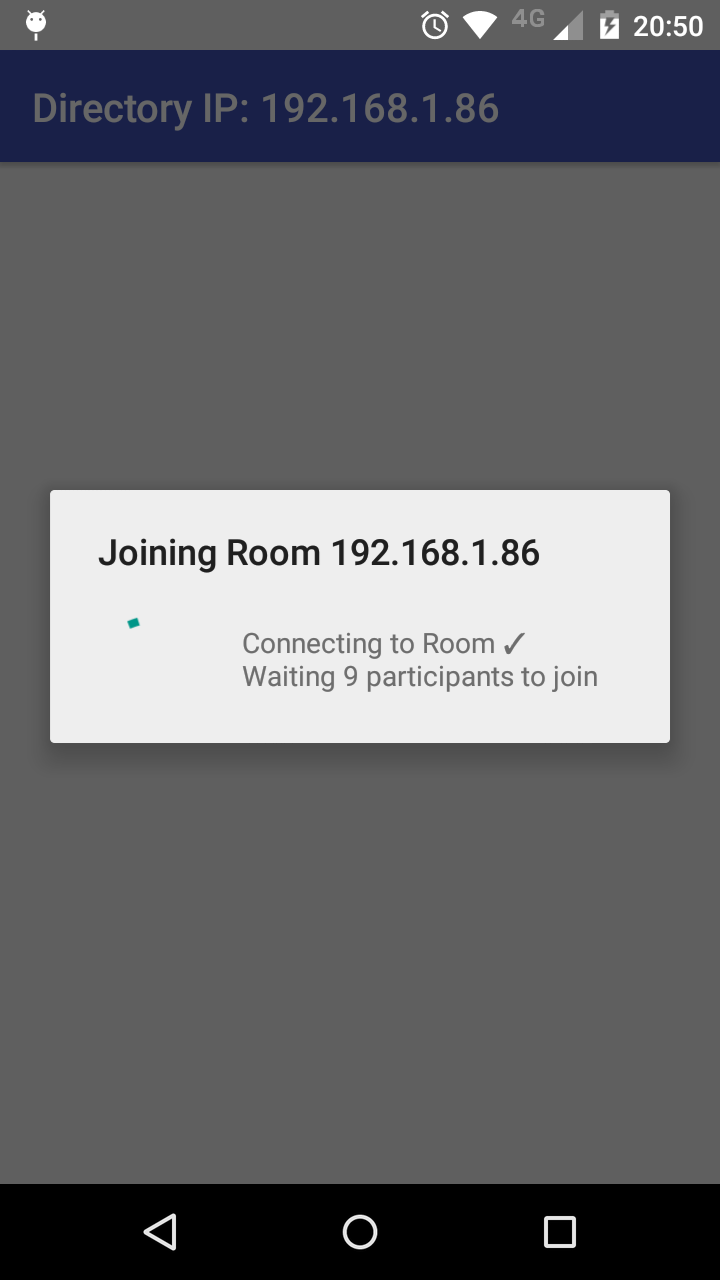
\includegraphics[width=\textwidth]{imagenes/mobile_connecting.png}
        \caption{Esperando conexión a Sala}
        \label{fig:mobile_waiting}
    \end{subfigure}
    ~
    \begin{subfigure}[b]{0.4\textwidth}
        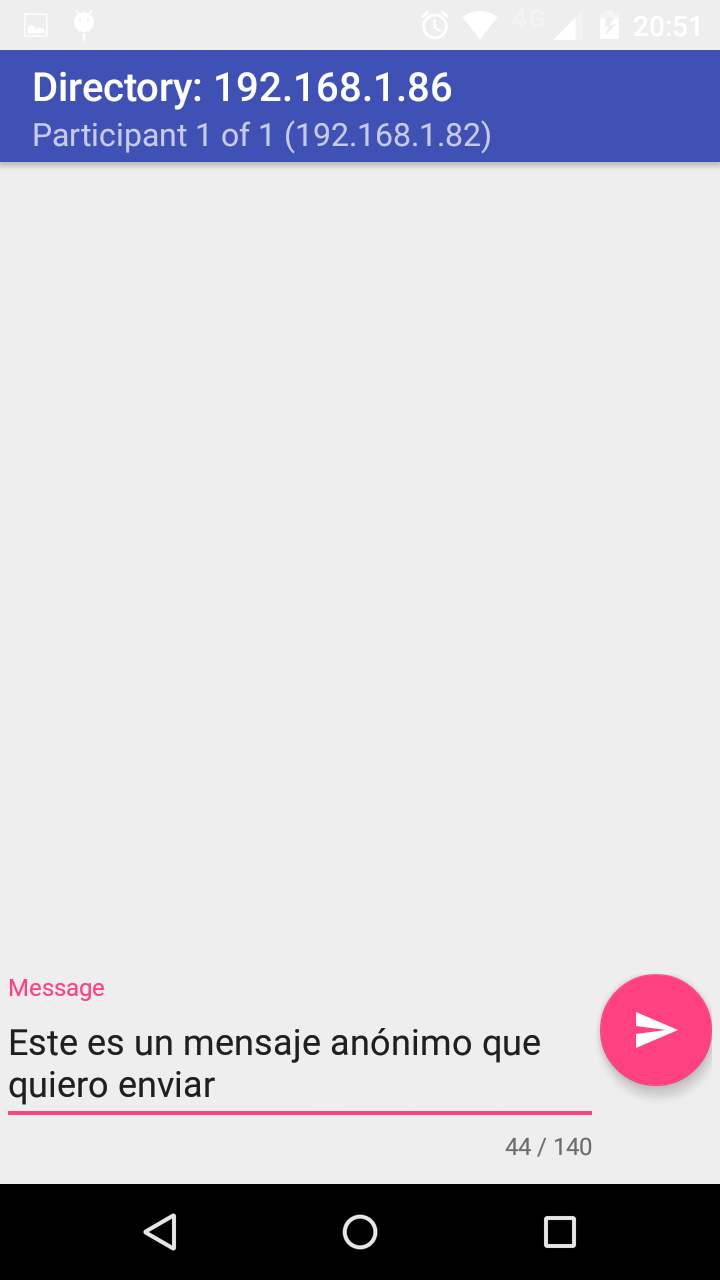
\includegraphics[width=\textwidth]{imagenes/mobile_message.png}
        \caption{Envío del mensaje a la sala}
        \label{fig:mobile_set_msg}
    \end{subfigure}
    \caption{Screenshots de Aplicación Móvil (parte 2)}\label{fig:mobile_screenshots_2}
\end{figure}

\section{Observación sobre tamaños de los mensajes}

Una observación importante a realizar de la implementación desarollada, es la 
cantidad de información (medida simplemente como el largo de los mensajes) que 
se envía en el protocolo. Se debe tomar como base el largo del mensaje 
original $m_i$ que cada participante debe comunicar. A esto se le debe agregar 
todas las \emph{zero-knowledge proofs} que necesita enviar, además de los \emph
{commitments}, los valores necesarios que debe comunicar para establecer 
llaves compartidas con todo el resto de la sala y considerar que en realidad 
lo que se envía en el protocolo es el mensaje $M_i$. A la suma de todos esos 
valores enviados le denotaremos $S_i$. Por último hay que considerar también 
que entre más participantes colisionen sus mensajes, más veces será necesario 
reenviar esta cantidad de información, debido a que se debe desarrollar un 
mayor número de rondas reales.

Para medir este sobrecosto que agrega el protocolo, se realizaron varios 
experimentos, donde se varió el tamaño del mensaje original que desea 
comunicar cada participante y se observó cuanta información se enviaba 
finalmente (por ronda) al resto de la sala. Importante notar que la cantidad 
de participantes presentes en la sala hace cambiar la cantidad de información a 
enviar, éste es un valor fijo (le envío a todos los participantes, la misma 
información), por lo que los resultados que se muestran en la Tabla \ref{table:message_sizes_table}, 
son por cada participante presente en la sala:

\begin{table}[h!]
\centering
\begin{tabular}[h!]{|c|c|c|}
\hline
$m_i$ (bytes) & $S_i$ (bytes) & $S_i / m_i$ \\ \hline
5                                   & 1633                               & 326.6       \\ \hline
10                                  & 1933                               & 193.3       \\ \hline
20                                  & 2624                               & 131.2       \\ \hline
40                                  & 3987                               & 99.7        \\ \hline
60                                  & 5288                               & 88.1        \\ \hline
80                                  & 6276                               & 78.5        \\ \hline
100                                 & 7459                               & 74.6        \\ \hline
120                                 & 8848                               & 73.7        \\ \hline
140                                 & 10281                              & 73.4        \\ \hline
200                                 & 14008                              & 70.1        \\ \hline
300                                 & 20200                              & 67.3        \\ \hline
\end{tabular}
\caption{Tamaño de mensajes enviados (por ronda)}
\label{table:message_sizes_table}
\end{table}

Cabe destacar, que entre más grande es el mensaje original a enviar, menor es 
el \emph{overhead} relativo que añade la ejecución del protocolo para asegurar 
anonimato y seguridad del sistema. Importante mencionar además que el tamaño 
del mensaje es determinado por el nodo directorio, en el comienzo del protocolo. 
El nodo directorio determina un largo máximo permitido para un mensaje a enviar 
durante la sesión actual. Independiente si algún participa envía un mensaje de largo menor a dicho 
máximo, el \emph{overhead} que presentará es el mismo que alguien que envía un 
mensaje con el largo máximo establecido por el nodo directorio.
